\newgeometry{margin=85pt}
\chapter*{Inteligencia Artificial Geoespacial}
\setcounter{chapter}{5} 
\setcounter{section}{0}
\addcontentsline{toc}{chapter}{Inteligencia Artificial Geoespacial}

La Inteligencia Artificia Geoespacial o \textit{Geospatial Artificial Intelligence} (GeoAI),
es el campo científico que surge de la combinación entre la innovación en la ciencia espacial, el consolidación de las aplicaciones de Inteligencia Artificial y el aumento de la capacidad de cómputo del hardware.  
El objetivo de la GeoAI es la extracción de conocimiento a partir de grandes volúmenes de datos espaciales.
Vivimos en la era de la digitalización y con ella se generan grandes volúmenes de datos, muchos de ellos de naturaleza geográfica,
ya que la mayoría de la información que nos rodea puede ser georreferenciada. En el artículo \cite{ESRI} escrito por ESRI, empresa que comercializa las aplicaciones ArcGIS 
(comentadas en la sección \ref{sec:herramientas}), se dice que “aproximadamente el 80\% de los datos de una organización tiene un componente de ubicación”.

En el análisis espacial, descrito en el capítulo anterior, podemos ubicar distintos eventos, pero con la GeoAI podemos conocer el por qué suceden dichos eventos.
Además, la GeoAI nos aporta una capacidad predictiva, permitiéndonos saber con antelación lo que va a suceder, muy útil por ejemplo en el campo de la meteorología, para la predecir fenómenos meteorológicos adversos.
También nos aporta una capacidad prescriptiva, permitiéndonos saber cómo actuar y tomar la decisión más correcta. Un ejemplo de ello son los patrones delictivos, 
cuya comprensión permite a las autoridades policiales gestionar de forma más eficiente sus recursos.

\section{Inteligencia Artificial}
La Inteligencia Artificial o \textit{Artificial Intelligence} (IA), tiene como objetivo que las máquinas sean capaces de realizar, sin ayuda, tareas que necesitarían intervención humana,
o lo que es lo mismo, simular la inteligencia humana en máquinas.
Existen dos campos destacados dentro de la IA: Aprendizaje Automático y Aprendizaje Profundo.

\subsection{Aprendizaje Automático}
El Aprendizaje Automático o \textit{Machine Learning} (ML), se basa en el uso de experiencias anteriores (instancias o ejemplos) para aprender de estas.
Cada instancia queda representada por una serie de características o atributos en diferentes clases o categorías,
y a partir de esa información, los sistemas obtienen un conocimiento, que dependiendo del uso que se le da, nos encontramos con tres grandes tipos de problemas:
\begin{itemize}
    \item Problemas de Regresión: el conocimiento se emplea para hacer predicciones sobre nuevos datos.
    \item Problemas de Clasificación: el conocimiento se emplea para decidir cuál es la clase a la que pertenecen los ejemplos nuevos sin etiquetar.
    \item Problemas de Clustering: el conocimiento se emplea para identificar clústeres, es decir, grupos de instancias agrupadas en base a alguna característica común.
\end{itemize} 

Según la forma en la que se utiliza la información con la que el ML aprende, nos encontramos cuatro grandes grupos:
\begin{itemize}
    \item Aprendizaje supervisado\\
    La información de la que se aprende se trata de datos que han sido etiquetados o clasificados previamente.
    A partir de estos, se busca el predecir y clasificar nueva información.
    \item Aprendizaje no-supervisado\\
    La información a partir de la que se aprende no está ni clasificada ni etiquetada previamente. 
    Tiene como objetivo el tratamiento de estos datos para conseguir una forma de describirlos.
    \item Aprendizaje semi-supervisado\\
    La información a partir de la que se aprende puede estar etiquetada o no etiquetada, 
    con el fin de conseguir información etiquetada y clasificada, suele ser una tarea difícil y costosa.
    \item Aprendizaje por refuerzo\\
    El aprendizaje se basa en interactuar con el entorno con el fin de maximizar unas recompensas,
    que serán mayores o menores en función de la forma en la que interactúa el sistema con el entorno. 
\end{itemize}

Un ejemplo aplicado de ML es el diagnóstico médico automatizado a partir de historiales médicos de pacientes. 
En este caso sería un problema de clasificación que emplea aprendizaje supervisado, en el que las instancias son los pacientes,
las características son los datos del historial médico y las cases indican si tiene o no alguna enfermedad. 

\subsection{Aprendizaje Profundo}
El Aprendizaje Profundo o \textit{Deep Learning} (DL), es un tipo de ML formado por algoritmos inspirados en el funcionamiento de nuestro cerebro,
empleando redes de neuronas interconectadas que intercambian información, conocidas como Redes Neuronales.
% En los problemas de DL la información de entrada no tiene una estructura definida, es decir, los ejemplos no están formados por un número de características fijo (numéricas o categóricas).
% Los modelos de DL extraen conocimiento de datos no estructurados como puede ser un correo electrónico, ficheros de texto, un tweet por ejemplo, audios, videos, imágenes, etc.

\subsubsection{Perceptrón}
\begin{figure}[H]
    \centering
    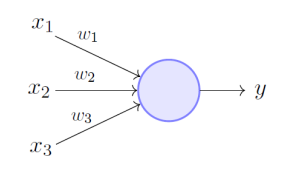
\includegraphics[width=0.40\textwidth]{Imagenes/GeoAI/perceptron.png}
    \caption{Modelo de un perceptrón} \label{fig:perceptron}
\end{figure}

Existen varios tipos de redes neuronales, el más simple es el \textit{Perceptrón}, formado por una sola neurona.
Como se observa en la figura \ref{fig:perceptron}, la neurona recibe un conjunto de valores de entrada \{$x_1, x_2, x_3$\}, 
que se combinan con el conjunto de pesos \{$w_1, w_2, w_3$\}, a lo que se le añade un bias \textit{b}, para producir una salida \textit{y}.
Por lo tanto, el \textit{Perceptrón} puede expresarse mediante la siguiente fórmula:
    
\[
    y =
    \begin{cases}
        1 & \text{si $x_1*w_1+x_2*w_2+x_3*w_3+b \geq 0$}\\
        0 & \text{en otro caso}
    \end{cases}
\]

\subsubsection{Red Neuronal Artificial}
\begin{figure}[H]
    \centering
    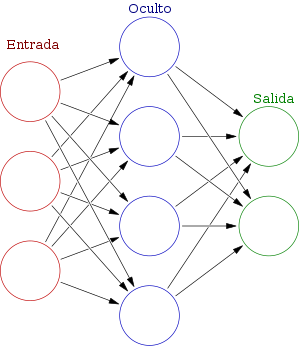
\includegraphics[width=0.35\textwidth]{Imagenes/GeoAI/red-neuronal.png}
    \caption{Red Neuronal Artificial} \label{fig:red-neuronal}
\end{figure}

La Red Neuronal Artificial está formada por un conjunto de perceptrones agrupados en capas, en donde la combinación de las salidas de la capa anterior y los parámetros del perceptrón,
producen la salida de este, que a su vez puede emplearse como entrada para una capa más profunda. En la figura \ref{fig:red-neuronal} vemos su arquitectura representada.
La primera capa o capa de entrada es la que recibe los datos con los que la red aprende, 
las capas intermedias o capas ocultas son las que van detectando distintos patrones de la información de entrada y
la última capa o capa de salida obtiene el resultado final, por ejemplo la clase a la que pertenece un ejemplo de entrada.
Cuando la red tiene un número elevado de capas ocultas, hablamos de redes neuronales profundas, que son las que realmente dan origen al término DL.

Según la función que define al \textit{Perceptrón}, teníamos que la salida puede ser 0 o 1. Para que la salida no sea binaria se emplean las funciones de activación.
Algunas de ellas las podemos ver en la siguiente tabla:
\begin{table}[H]
    \centering
    \begin{tabular}{|c|c|c|}
    \hline
                         & Función                                      & Rango                  \\
    \hline
    Sigmoidea            & $\sigma(z) = \frac{1}{1 + e^{-z}}$            & [0,1]                 \\
    \hline
    Tangente hiperbólica & $tanh(z) = \frac{e^z - e^{-z}}{e^z + e^{-z}}$ & [-1,1]                 \\
    \hline
    ReLU                 & $\text{ReLU = max} (0, z)$                    & [0, +$\infty$]          \\
    \hline
    Lineal               & $g(z) = z$                                    & [-$\infty$, +$\infty$]  \\
    \hline
    \end{tabular}
\end{table}
en donde $z = \displaystyle \sum_{i} w_i * x_i - b$.\\

Para que la red sea capaz de aprender, tiene que ajustar los parámetros de la red (pesos y bias) de cada una de las neuronas, minimizando la función de coste,
que suele ser el error cuadrático medio. Para ello, se emplea el algoritmo del descenso por gradiente.
Este algoritmo de optimización se basa en el concepto de que la derivada de una función es la pendiente de la tangente en ese punto.
Cuando se encuentra en un máximo o un mínimo, está pendiente se evalúa a cero.
Para aplicar este algoritmo a toda la red y actualizar sus parámetros se realiza una propagación hacia atrás o \textit{backpropagation}.

\subsubsection{Red Neuronal Convolucional}
Las redes neuronales convolucionales o \textit{Convolutional Neural Networks} (CNN), son un tipo de red neuronal artificial diseñada para que trabaje con matrices de dos o tres dimensiones,
normalmente imágenes. La forma que tiene la red de interactuar con esta información es utilizando las operaciones de convolución entre dos matrices.

\begin{figure}[H]
    \centering
    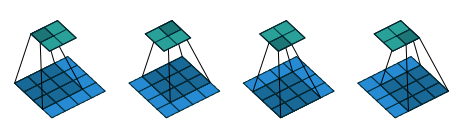
\includegraphics[width=0.85\textwidth, height=0.15\textheight]{Imagenes/geoAI/convolucion.png}
    \caption{Convolución entre dos matrices} \label{fig:convolucion}
\end{figure}

Una convolución es una técnica que aplica un filtro \textit{g} sobre los píxeles de una imagen, por ejemplo, para desenfocarla o para detectar bordes.
En el procesamiento de imágenes, \textit{g} se denomina función kernel o matriz de convolución con dimensión \textit{m} x \textit{n}, 
que recorre la imagen de entrada realizando una combinación de los coeficientes de la función Kernel y las intensidades de los píxeles de la imagen.
Podemos observar dicho proceso en la figura \ref{fig:convolucion}.
Formalmente, la convolución entre \textit{g} y una imagen \textit{f} de dimensión \textit{M}x \textit{N} se escribe como
\begin{equation}
    (g * f)(x,y) = \displaystyle\sum_{i=-a}^a \sum_{j=-b}^b g(s,t)f(x+i,y+j)\nonumber
\end{equation}

La CNN recibe una imagen o capa ráster como entrada, a la que aplica una serie de convoluciones a través de las capas convolucionales,
cuyas neuronas tienen los valores de la función kernel como pesos. 
Posteriormente, se realiza la activación de la neurona, y si la imagen resultante sigue teniendo un tamaño elevado, se vuelve a repetir el proceso (convoluciones + activación).
Las convoluciones permite a la red extraer características, desde bordes en las primeras capas hasta formas más complejas en las capas profundas.  
También existen otras capas para acelerar el proceso de reducir el tamaño de los valores de salida, llamadas capas pooling.
Estas agrupan la salida de la neurona, produciendo un único valor. Para ello se suele emplear la media aritmética o máximo.

\begin{figure}[H]
    \centering
    \subfigure[Clasificación]{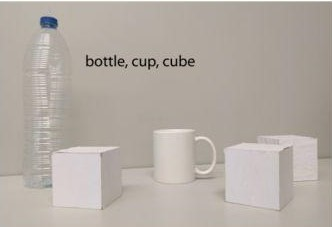
\includegraphics[width=0.35\columnwidth]{Imagenes/GeoAI/clasificacion.jpeg}}
    \subfigure[Detección]{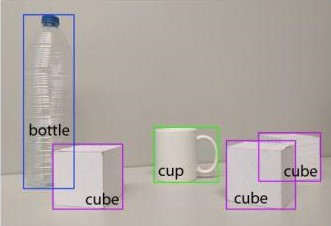
\includegraphics[width=0.35\columnwidth]{Imagenes/GeoAI/deteccion.jpeg}}
    \subfigure[Segmentación semántica]{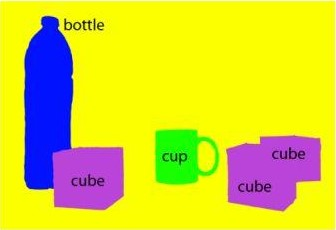
\includegraphics[width=0.35\columnwidth]{Imagenes/GeoAI/segmentacion-semantica.jpeg}}
    \subfigure[Segmentación de instancias]{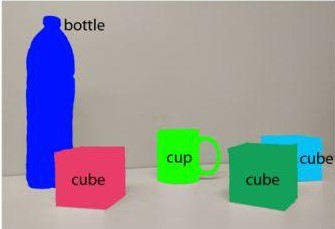
\includegraphics[width=0.35\columnwidth]{Imagenes/GeoAI/segmentacion-instancias.jpeg}}
    \caption{Algoritmos de procesamiento de imágenes} \label{fig:preprocesamiento-imagenes} 
\end{figure} 

Las CNN han permitido grandes avances en el procesamiento de imágenes, permitiendo resolver problemas de segmentación, clasificación y detección de objetos en imágenes,
ls cuales podemos ver en la figura \ref{fig:preprocesamiento-imagenes}.
La clasificación asigna una clase a la imagen de entrada, dentro de las diferentes clases que el algoritmo conoce.
La detección de objetos supone un paso más y no nos indica solamente que la imagen contiene unos objetos, sino que también dice donde se encuentran esos objetos dentro de la imagen.
Para ello delimita cada objeto con un rectángulo conocido como bounding box, que se ajusta al máximo a los límites del objeto.
En ocasiones el empleo de bounding box no es suficiente, ya que hay problemas en los que se requiere detectar todos los píxeles del objeto.
Es estos casos se emplea la segmentación, que puede ser de tipo semántica cuando detecta todos los píxeles de la imagen correspondientes a cada clase.
También existe la segmentación de instancias, que diferencia las instancias dentro de las clases detectadas. 

\section{Inteligencia Artificial con datos espaciales}
A continuación, comentaremos algunos ejemplos de algoritmos de IA aplicados sobre datos espaciales. 
Estos tipos de datos nos permites tener mayor información de las instancias empleadas para aprender, 
ya que además de estar formadas por un conjunto de atributos, cuentan con una geometría que les define en el espacio.

\subsection{Modelos de aprendizaje automático}

\subsubsection{Clustering con k-means}
\textit{K-means} es un algoritmo de clustering no-supervisado. 
La identificación de clústeres se realiza en función de la distancia, en el que cada clúster queda definido en base de la proximidad espacial de las instancias.

\begin{figure}[H]
    \centering
    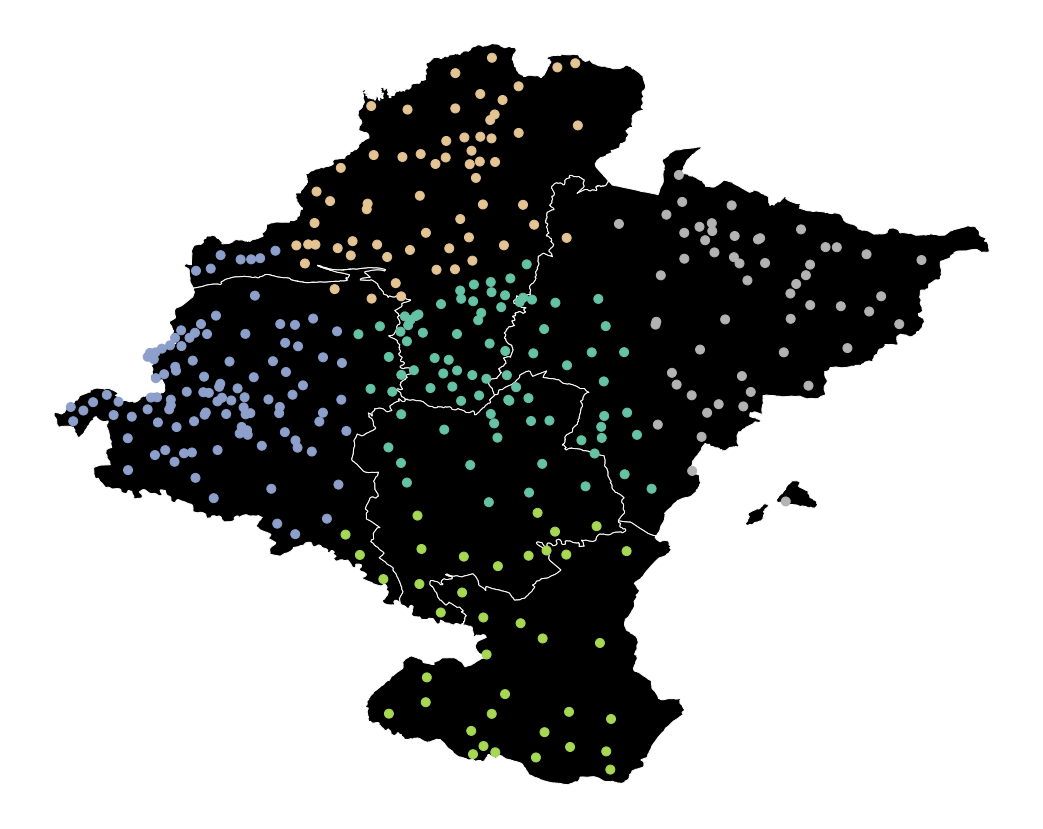
\includegraphics[width=0.65\textwidth]{Imagenes/GeoAI/kmeans.png}
    \caption{Clústeres municipios en base a la distancia} \label{fig:clusteres-municipios}
\end{figure}

En la figura \ref{fig:clusteres-municipios} se observa el resultado de aplicar el algoritmo de k-means, con k igual a 5, basado en la distancia sobre los municipios de Navarra.
El mapa base está formado por las merindades de Navarra (Pamplona, Estella, Olite, Sangüesa y Tudela)
y se puede apreciar cierta coincidencia entre los clústeres generados y el área que ocupa las merindades.

\begin{figure}[H]
    \centering
    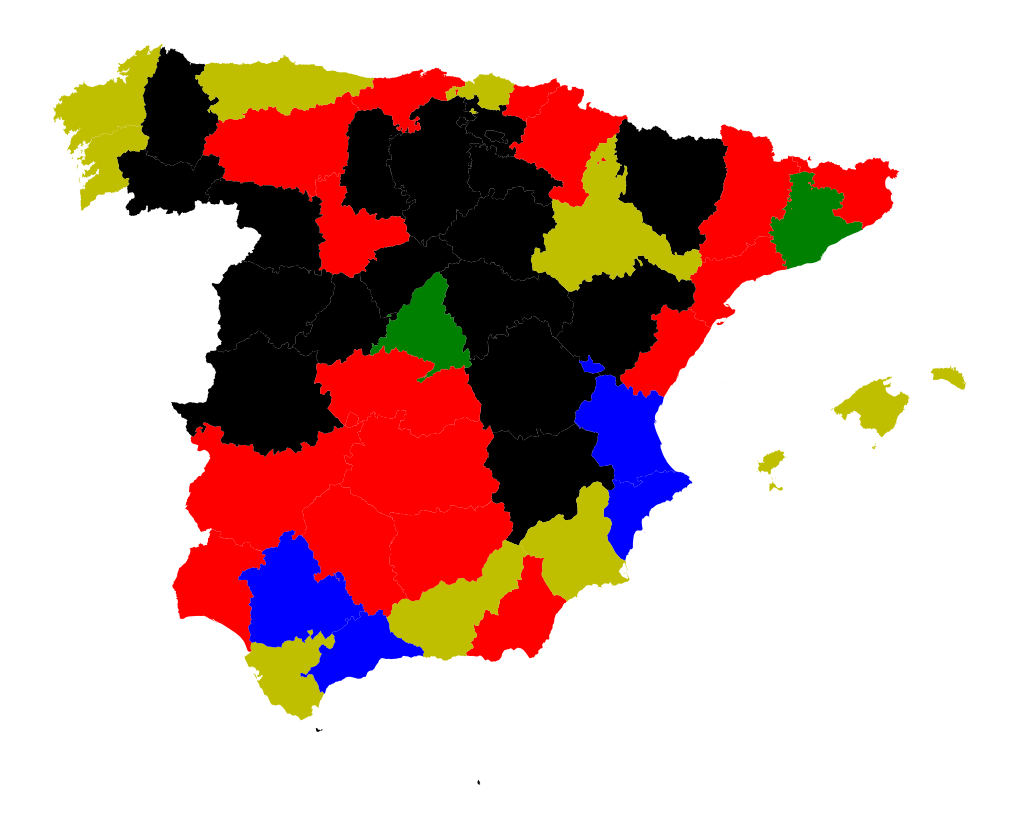
\includegraphics[width=0.84\textwidth]{Imagenes/GeoAI/kmeans-atributo.png}
    \caption{Clústeres provincias en base a la población} \label{fig:clusteres-provincias}
\end{figure}

\begin{table}[H]
    \centering
    \begin{tabular}{|c|c|c|}
    \hline
    Provincia         & Habitantes & cluster \\
    \hline
    Madrid            & 6769113.0  &  1      \\
    \hline
    Barcelona         & 5641485.0  &  1      \\
    \hline
    València/Valencia & 2589308.0  &  2      \\
    \hline
    Sevilla           & 1960257.0  &  2      \\
    \hline
    Alacant/Alicante  & 1904362.0  &  2      \\
    \hline
    Málaga            & 1711693.0  &  2      \\
    \hline
    Murcia            & 1522640.0  &  3      \\
    \hline
    Cádiz             & 1259339.0  &  3      \\
    \hline
    \end{tabular}
\end{table}

También existe la identificación de clústeres en función de la “proximidad estadística”, es decir,
en base a una determinada significancia estadística de alguno de los atributos numéricos.
Incluso podemos emplear más de un atributo estadístico, asignando un peso a cada uno de ellos.
En la figura \ref{fig:clusteres-provincias} se observa el resultado de aplicar k-means, con k igual a 5, basado en el número de habitantes de cada provincia de España.
En concreto se ha obtenido el número total de habitantes por provincia en el primer semestre de 2022 (Fuente: Instituto Nacional de Estadística).
Podemos ver en la tabla el top 8 de las provincias con mayor número de habitantes y el clúster en el que se encuentran.

El uso del clustering de datos espaciales es común para discretizar características que se vayan a emplear en otros modelos.
Por ejemplo, según la agrupación de provincias en base a la población reflejada en la figura \ref{fig:clusteres-provincias},
podemos asociar a cada provincia una población “Muy Baja”, “Baja”, “Media”, “Alta” o “Muy Alta”.
En el estudio \cite{COVID} se emplea esta técnica con el fin de entrenar una red neuronal que devuelve el número de contagios totales de COVID-19
que se iba a tener al día siguiente.  

\subsubsection{Clasificación con máquinas de vector de soporte}
El modelo de Máquina de Vector de Soporte o \textit{Support Vector Machine} (SVM) es un algoritmo de clasificación supervisado.
Dado un conjunto separable de \textit{n} ejemplos de entrenamiento, cada uno de ellos con \textit{d} atributos y que pertenecen a la clase +1 o -1, 
existe infinitos hiperplanos que los separan. La regresión lineal o logística devuelve uno de los hiperplanos que separa los ejemplos por clase.
La diferencia con SVM es que este encuentra el hiperplano más óptimo, que es aquel en el que el margen es de tamaño máximo.
El margen es la distancia mínima entre el hiperplano y el(los) ejemplo(s) más cercano(s) de cualquier clase.

\begin{figure}[H]
    \centering
    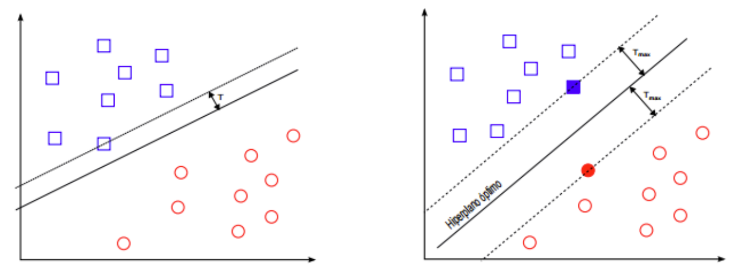
\includegraphics[width=0.65\textwidth]{Imagenes/GeoAI/SVM.png}
    \caption{Hiperplano en el modelo SVM} \label{fig:svm}
\end{figure}

En la figura \ref{fig:svm} vemos dos ejemplos de hiperplanos que separan los ejemplos según su clase. El de la derecha resulta ser el más óptimo, ya que es el de margen con más tamaño, 
y además es equidistante a los ejemplos de ambas clases (ejemplos resaltados). Estos ejemplos son los vectores de soporte,
y se denominan así en lugar de puntos porque tienen tantos elementos como dimensiones tenga nuestro espacio de entrada.
En este caso sería d-dimensiona ya que hemos definido a cada ejemplo con \textit{d} atributos.

\begin{figure}[H]
    \centering
    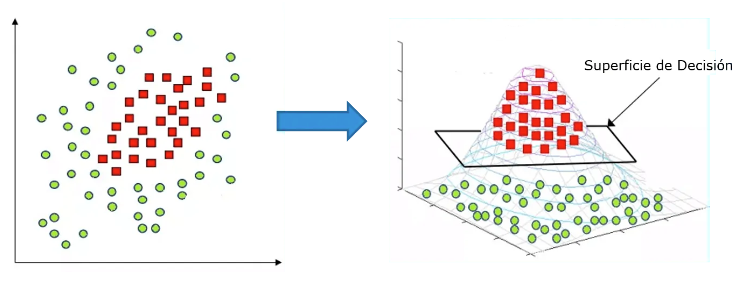
\includegraphics[width=0.65\textwidth]{Imagenes/GeoAI/kernel-SVM.png}
    \caption{Función Kernel en el modelo SVM} \label{fig:kernel-svm}
\end{figure}

No siempre nos encontramos con clases linealmente separables. 
En esos casos podemos emplear las funciones kernel para que sí lo sean.
Consisten en expandir las dimensiones del espacio original para que las clases sean linealmente separables.
En la figura \ref{fig:kernel-svm} vemos que los conjuntos de ejemplos de cada clase no son linealmente separables en dos dimensiones, pero sí que lo son si convertimos el espacio estudiado a 3 dimensiones.

En cuanto al empleo de los SVM en GIS, el modelo se emplea para varios objetivos, ya que soluciona tanto para problemas de regresión como de clasificación.
Por ejemplo, podemos seleccionar atributos numéricos de datos espaciales como características de los ejemplos con los que entrenamos al SVM.
En este caso podemos emplear otro atributo como clase con la que se etiqueta cada ejemplo.
Si ese atributo tiene valor continuo, como por ejemplo la altitud, estamos ante un problema de regresión.
Si el atributo toma valores en un conjunto finito y discreto, como por ejemplo el uso del suelo, estamos ante un problema de clasificación.
También los SVM se emplean la clasificación de imágenes, en dónde las características de cada ejemplo corresponden a las coordenadas de cada punto.
En notebook \cite{Kaggle} de Kaggle, vemos un ejemplo de SVM como clasificador de imágenes según su color.
Kaggle es la plataforma educativa más grande del mundo en materia de Ciencia de Datos 
y los notebooks son entornos de Python que permite disponer bloques de texto y de código, estos últimos comparten las mismas variables pero se pueden ejecutar de forma independiente.

\begin{figure}[H]
    \centering
    \subfigure[Imagen satelital original]{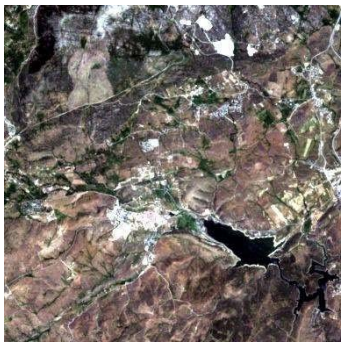
\includegraphics[width=0.28\columnwidth]{Imagenes/GeoAI/ejemplo-SVM.png}}
    \subfigure[Ejemplos entrenamiento]{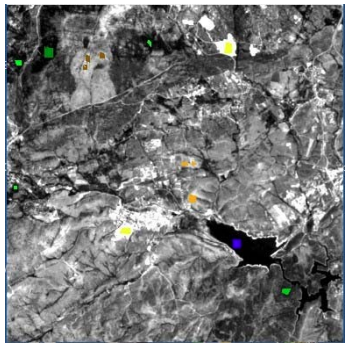
\includegraphics[width=0.28\columnwidth]{Imagenes/GeoAI/ejemplo-SVM1.png}}
    \subfigure[Imagen segmentada]{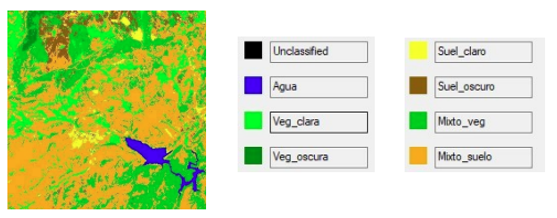
\includegraphics[width=0.75\textwidth, height=0.20\textheight]{Imagenes/GeoAI/ejemplo-SVM2.png}}
    \caption{Segmentación imagen satelital mediante SVM} \label{fig:ejemplo-SVM} 
  \end{figure} 

Por último, los SVM se emplean en segmentación de imágenes, cuyo ejemplo podemos ver en la figura \ref{fig:ejemplo-SVM}, en donde se recoge como entrada una imagen ráster capturada por un satélite.
A partir de esa imagen se etiquetan algunos píxeles con las etiquetas definidas que sirven como entrenamiento del modelo SVM.
Finalmente se realiza la clasificación del resto de píxeles de la imagen.

\subsection{Modelos de aprendizaje profundo}
Durante 2021, la empresa ESRI ha desarrollado 25 modelos de DL que los ofrece como \textit{Saas (Software as a Service)} \cite{DeepLearningArcGIS}.
Los modelos se emplean para el reconocimiento y la clasificación de objetos en imágenes aéreas o satelitales. 
Algunos de los modelos clasifican infraestructuras como carreteras o redes eléctricas, otros detectan personas, y también hay varios que están relacionados con el agua.
Algunos ejemplos de ellos son:

\subsubsection{Clasificación de la cobertura terrestre en imágenes de alta resolución}
El término de cobertura terrestre hace referencia al material físico del que se compone la superficie terrestre. 
Existe un inventario dirigido por la Agencia Europea de Medio Ambiente (AEMA) sobre la cobertura terrestre y el uso del territorio en la Unión Europea, denominado \textit{CORINE Land Cover (CLC)}.
El CLC distingue entre zonas forestales, masas de agua y superficies artificiales, como zonas urbanas, zonas industriales, superficies agrarias, entre otros. 
En el artículo \cite{CLC} se define en detalle cada una de las 44 clases de la cobertura terrestre propuestas por CLC. 

\begin{figure}[H]
    \centering
    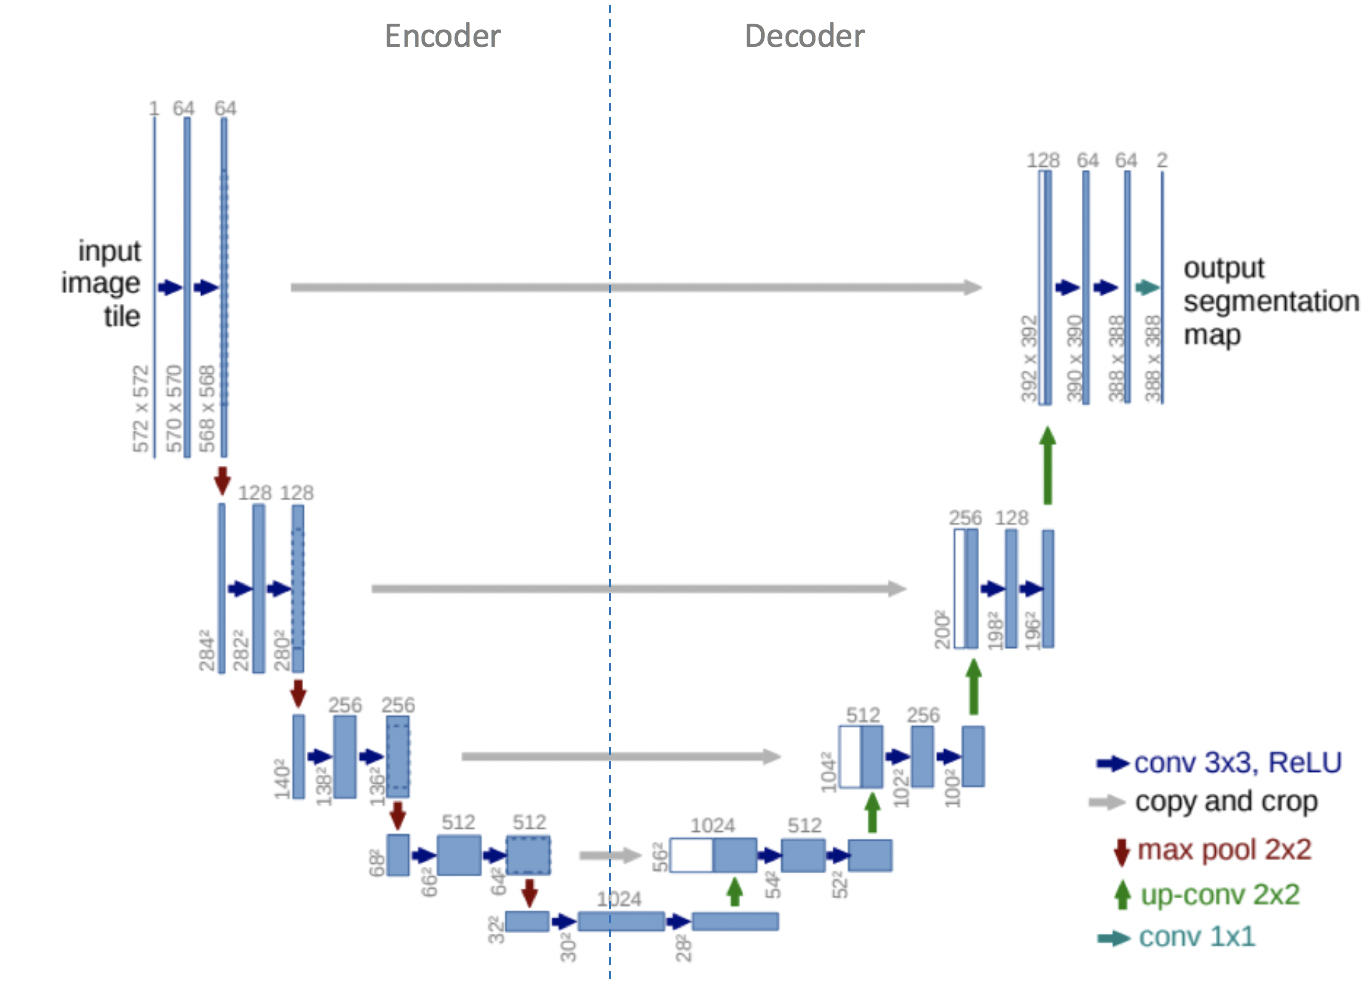
\includegraphics[width=0.80\textwidth]{Imagenes/GeoAI/unet.png}
    \caption{Arquitectura modelo U-net} \label{fig:u-net}
\end{figure}

El modelo toma como entrada un conjunto de imágenes ráster y genera la cobertura terrestre empleando las clases del CLC. 
Para ello, emplea el algoritmo de segmentación semántica \textit{U-net}, cuya arquitectura podemos observar en la figura \ref{fig:u-net}.
\textit{U-net} utilizó por primera vez para la segmentación de imágenes biomédicas \cite{Ronneberger2015}, se compone de una red codificadora seguida de una red decodificadora.
La red codificadora es una red de clasificación preentrenada como \textit{VGG/ResNet} en la que se aplican capas de convolución seguidas de capas pooling empleando el máximo (maxpool),
para codificar la imagen de entrada en diferentes características, que finalmente quedan contenidas en un array de 1024 valores.
Para proyectar esas características a un espacio de mayor dimensión se emplea la red decodificadora proyecta, 
en donde se realizan operaciones seguidas de convolución ascendente, también conocida como convolución transpuesta. 

\begin{figure}[H]
    \centering
    \subfigure[Convolución]{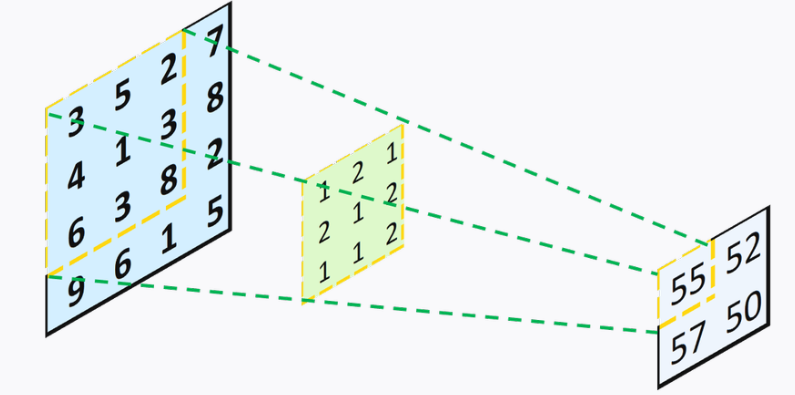
\includegraphics[width=0.35\columnwidth]{Imagenes/geoAI/ejemplo-convolucion.png}}
    \subfigure[Convolución transpuesta]{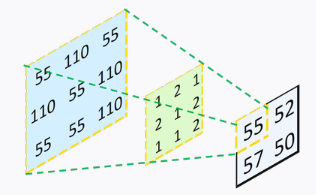
\includegraphics[width=0.30\columnwidth]{Imagenes/geoAI/ejemplo-convolucion-transpuesta.png}}
    \caption{Operaciones de convolución} \label{fig:operaciones-convolucion} 
\end{figure} 

En la figura \ref{fig:operaciones-convolucion} vemos la diferencia entre la operación de convolución y la de convolución transpuesta.
En la convolución transpuesta aumentamos el tamaño de la matriz, pero los valores originales no se restauran si se emplea la misma función Kernel.
Si se quiere restaurar la matriz original, se debe emplear otra función kernel, que en el caso de las CNN se inicia con números aleatorios y se modifica a medida que la red aprende.
En el artículo \cite{ConvolucionTranspuesta} explica una forma de realizar la operación de convolución transpuesta empleando una matriz de convolución rellenada de ceros,
en lugar de emplear una matriz cuadrada como las de la figura \ref{fig:operaciones-convolucion}.

\begin{figure}[H]
    \centering
    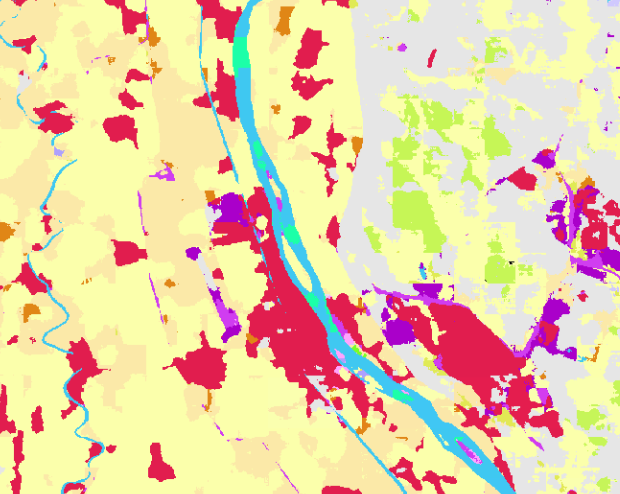
\includegraphics[width=0.50\textwidth]{Imagenes/GeoAI/cobertura-terrestre.png}
    \caption{Cobertura terrestre} \label{fig:cobertura-terrestre}
\end{figure}

La salida del modelo se muestra en la figura \ref{fig:cobertura-terrestre}, correspondiente a una imagen con la cobertura terrestre de la imagen original.

\subsubsection{Detección de personas en imágenes de drones}
Los drones se utilizan para capturar imágenes de alta resolución, muy útiles para que los equipos de emergencias inspeccionen el terreno en caso de desastres naturales.
En estos casos es posible encontrar supervivientes, pero la detección de personas de forma manual requiere mucho tiempo y además es propensa a errores humanos.
Por ello, resulta interesante contar con un modelo que toma como entrada un conjunto de imágenes de drones de alta resolución (de 1 a 5 cm) y 
devuelve los bluonding box que envuelven a las personas que aparecen en cada imagen.
Para ello, el modelo emplea el algoritmo de detección de objetos \textit{FasterRCNN}, que forma parte de la familia \textit{R-CNN}.

\begin{itemize}
    \item R-CNN \\
    \begin{figure}[H]
        \centering
        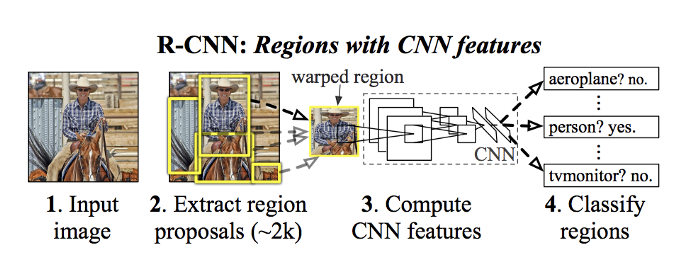
\includegraphics[width=0.70\textwidth]{Imagenes/GeoAI/RCNN.png}
        \caption{R-CNN} \label{fig:RCNN}
    \end{figure}
    La Red Neuronal Convolucional basada en Regiones o \textit{Region-based Convolutional Neural Networks} (R-CNN) presenta el siguiente flujo, el cual se muestra en la figura \ref{fig:RCNN}.
    \begin{enumerate}
        \item Se realiza una extracción de regiones de interés de una imagen de entrada.
        Para ello se puede emplear el algoritmo \textit{Selective Search}, que utiliza un método de segmentación exagerada de la imagen basada en la intensidad de los píxeles.
        \item Cada región se pasa a una CNN para extraer las características.
        \item Por último, la información obtenida por la CNN es interpretada por un conjunto de \textit{SVMs}, en donde cada una de estas, esta entrenada para detectar una sola clase.
    \end{enumerate}
    
    Este modelo contiene ciertas limitaciones. La más clara es el tiempo necesario para el entrenamiento del modelo completo, ya contiene varias etapas, por lo que es un proceso largo y complicado. 
    Además, es necesario evaluar todas y cada una de las regiones, una por una, con la CNN, lo que aumenta más el tiempo de entrenamiento.
    Para solucionar las limitaciones del modelo diseñado en 2014, en 2015 se introduce una extensión de la primera versión de R-CNN, llamada Fast R-CNN.
    
    \item Fast R-CNN \\
    \begin{figure}[H]
        \centering
        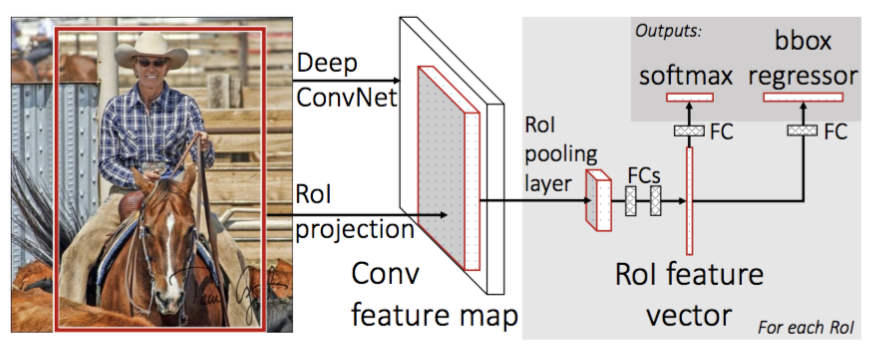
\includegraphics[width=0.70\textwidth]{Imagenes/GeoAI/FastRCNN.png}
        \caption{Fast R-CNN} \label{fig:FastRCNN}
    \end{figure}
    En la arquitectura de Fast R-CNN que se muestra en la figura \ref{fig:FastRCNN}, la primera diferencia que se puede observar es que,
    la entrada al modelo es la imagen sobre la que detectar los objetos y también, las regiones propuestas.
    Dentro de la CNN, una capa pooling se encarga de extraer un vector de un tamaño fijo. 
    Cada uno de los vectores de salida de la capa pooling se introduce a una secuencia de capas, una capa softmax (función de activación para problemas multiclase) 
    que produce las confianzas de salida para cada una de las regiones y otra que devuelve las posiciones de las bounding boxes.
    Pero todavía se utiliza \textit{Selective Search} como el algoritmo de propuesta de posibles regiones de interés, el cual, puede tardar hasta 2s por imagen y produce
    una gran cantidad de regiones posibles, lo que provoca una pérdida de rendimiento en el modelo de detección.

    \item Faster R-CNN \\
    \begin{figure}[H]
        \centering
        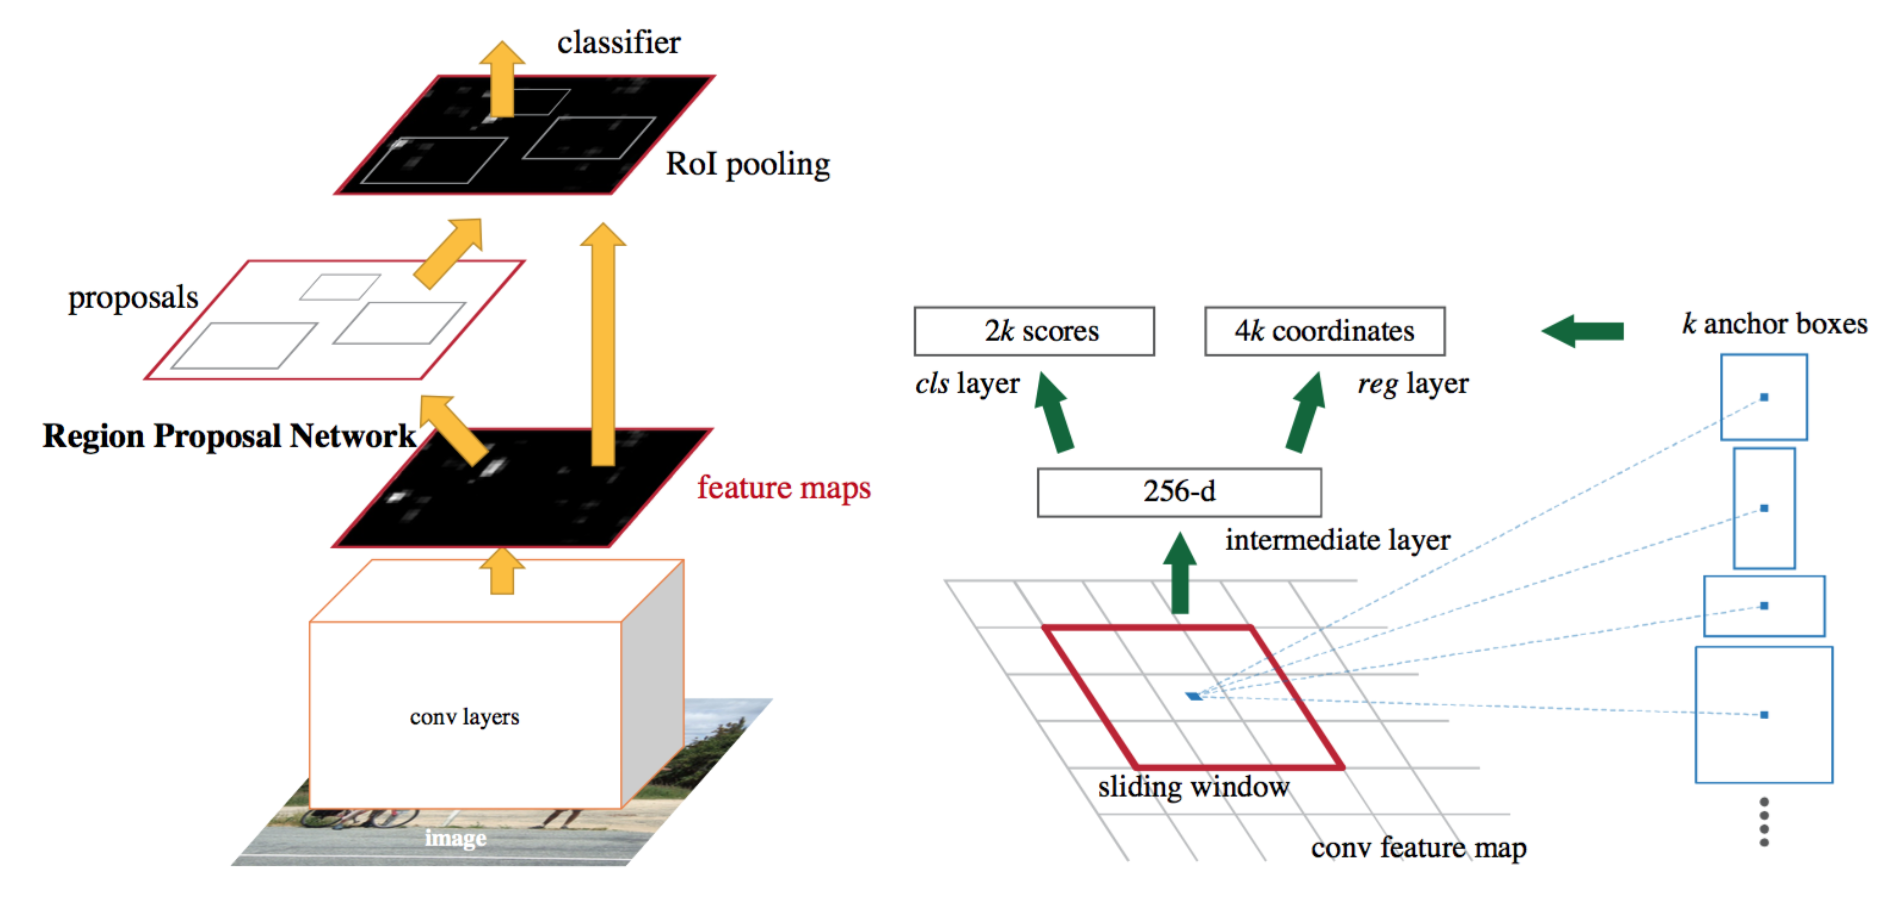
\includegraphics[width=0.80\textwidth]{Imagenes/GeoAI/FasterRCNN.png}
        \caption{Faster R-CNN} \label{fig:FasterRCNN}
    \end{figure}
    En 2016, propuso un nuevo modelo llamado Faster R-CNN, en el que se integra el proceso de proponer y refinar las regiones de interés dentro del entrenamiento del
    modelo denominado red de proposición de regiones (RPN).
    La RPN actúa sobre la misma CNN con la que trabaja Fast R-CNN para extraer la información sobre la imagen original. 
    Para ello, se utiliza una pequeña red que se desplaza sobre la salida de las capas convolucionales del modelo.
    Esta pequeña red toma como entrada una ventana de dimensiones n x n sobre la matriz de características recibida como entrada.
    Cada una de las ventanas se mapea a un vector pequeño (256 elementos o 512 elementos) y cada uno de estos se conecta a
    dos capas de manera completa, una para para generar las bounding boxes (reg) y
    otra para la probabilidad que la bounding box tenga o no un objeto (cls).
\end{itemize}

\begin{figure}[H]
    \centering
    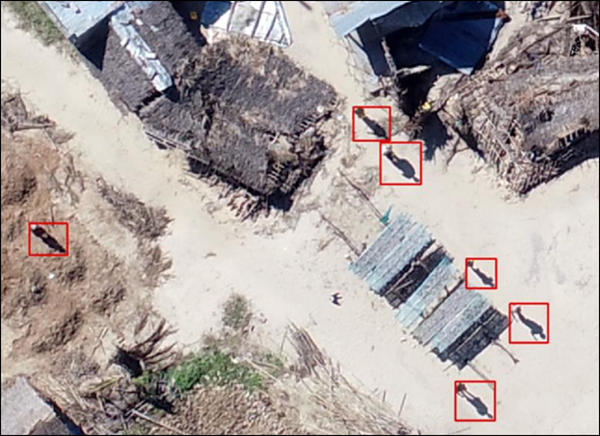
\includegraphics[width=0.50\textwidth]{Imagenes/GeoAI/deteccion-personas.png}
    \caption{Detección de personas en imagen de dron} \label{fig:deteccion-personas}
\end{figure}

La salida del modelo se muestra en la figura \ref{fig:deteccion-personas}, correspondiente a una los bluonding box que envuelven a las personas que aparecen en la imagen original tomada desde un dron.
